\section{Dataset and Exploratory Analysis}
\label{sec:data}

\subsection{METR-LA}
METR-LA~\cite{jagadish2014,li2018dcrnn} contains 5-minute average speeds from
$N{=}207$ loop detectors on Los Angeles County freeways, from 1~March to 27~June
2012 ($T{=}34{,}272$ steps; Table~\ref{tab:data}). It ships with sensor
coordinates and 295,374 directed road-network distances, of which 11,753 are
between sensors in the dataset. The HDF5 file was written by pandas~0.15, so we
read its arrays directly with \texttt{h5py}.

\begin{table}[t]
\centering
\caption{Dataset summary (computed by \texttt{scripts/run\_eda.py}).}
\label{tab:data}
\begin{tabular}{ll}
\toprule
Sensors / time steps & 207 / 34,272 (119 days, 5 min) \\
Missing readings (value $=0$) & 8.11\,\% (per sensor 6.3--20.1\,\%) \\
Observed speed mean $\pm$ std & 58.5 $\pm$ 13.0 mph (median 63.2) \\
Readings $<$ 40 mph (congested) & 10.9\,\% \\
Skewness & $-1.99$ \\
Graph non-zeros (incl.\ self-loops) & 1,722 (1,515 directed edges) \\
One-way edges & 73.3\,\% \\
Split (windows) & 23,974 / 3,425 / 6,850 \\
\bottomrule
\end{tabular}
\end{table}

\subsection{Data quality}
Missing observations are encoded as $0$\,mph, which is physically implausible on a
freeway. They make up 8.1\,\% of readings. Fig.~\ref{fig:missing} shows two
mechanisms: network-wide outages (vertical stripes, e.g.\ 26--27~March, when
$>$50\,\% of readings are missing) and long single-sensor failures (the median
sensor's longest gap is 381 steps, about 32\,h). Speeds are capped at 70\,mph by the
sensors' processing. We therefore (i) mask zero targets out of every loss and metric,
(ii) never impute labels, and (iii) use only \emph{causal} forward-filling (last
observation carried forward) when building features. Interpolation would use future
values.

\begin{figure*}[t]
\centering
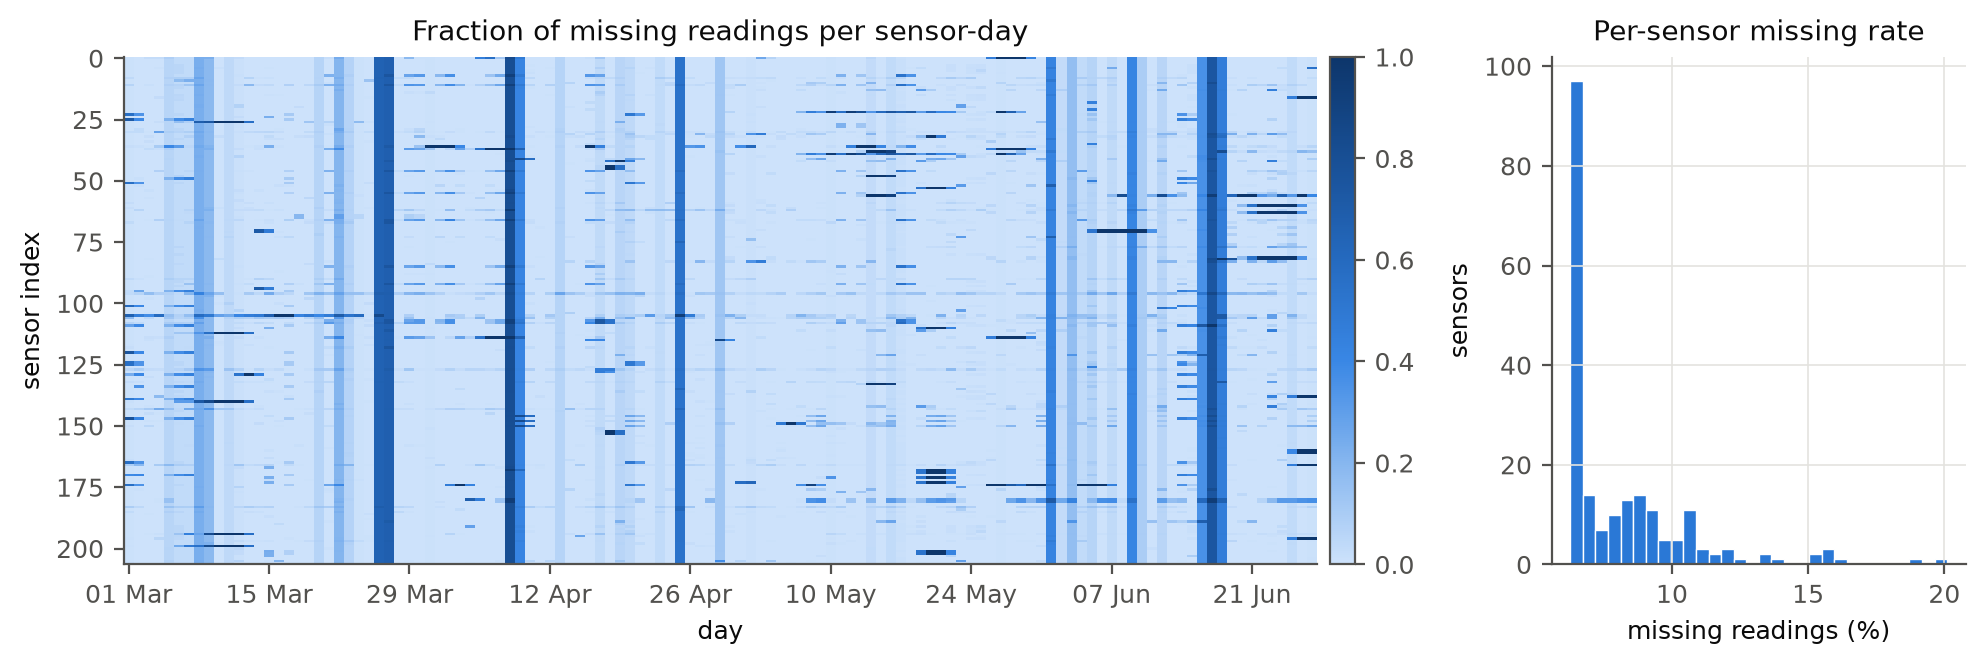
\includegraphics[width=0.85\textwidth]{eda_missingness.png}
\caption{Missingness. Left: fraction of zero readings per sensor-day. Vertical
stripes are network outages; horizontal streaks are sensor failures. Right:
distribution of per-sensor missing rates.}
\label{fig:missing}
\end{figure*}

\subsection{Temporal structure}
Weekday speeds show a pronounced evening rush hour (network mean 45.2\,mph at
17:30) and a weaker morning dip, while weekends are flat (minimum 56.8\,mph;
Fig.~\ref{fig:profile}). The autocorrelation function (Fig.~\ref{fig:acf}) is
0.86 at lag 5\,min and 0.57 at 1\,h. It peaks every 24\,h, with the 168\,h peak
(0.40) above the 24\,h peak (0.36), so the seasonality is weekly. Subtracting each
sensor's weekly profile (fitted on training data) removes the daily peaks: the
24\,h ACF falls from 0.36 to 0.07. The residual \emph{anomaly} is a short-memory
process (ACF 0.41 at 1\,h). This additive decomposition, speed = weekly profile +
anomaly, motivates several features. Augmented Dickey--Fuller
tests~\cite{dickey1979} reject a unit root for all ten sampled sensors
($p<10^{-24}$), so the series need no differencing; their non-stationarity is
seasonal, not a stochastic trend.

\begin{figure*}[t]
\centering
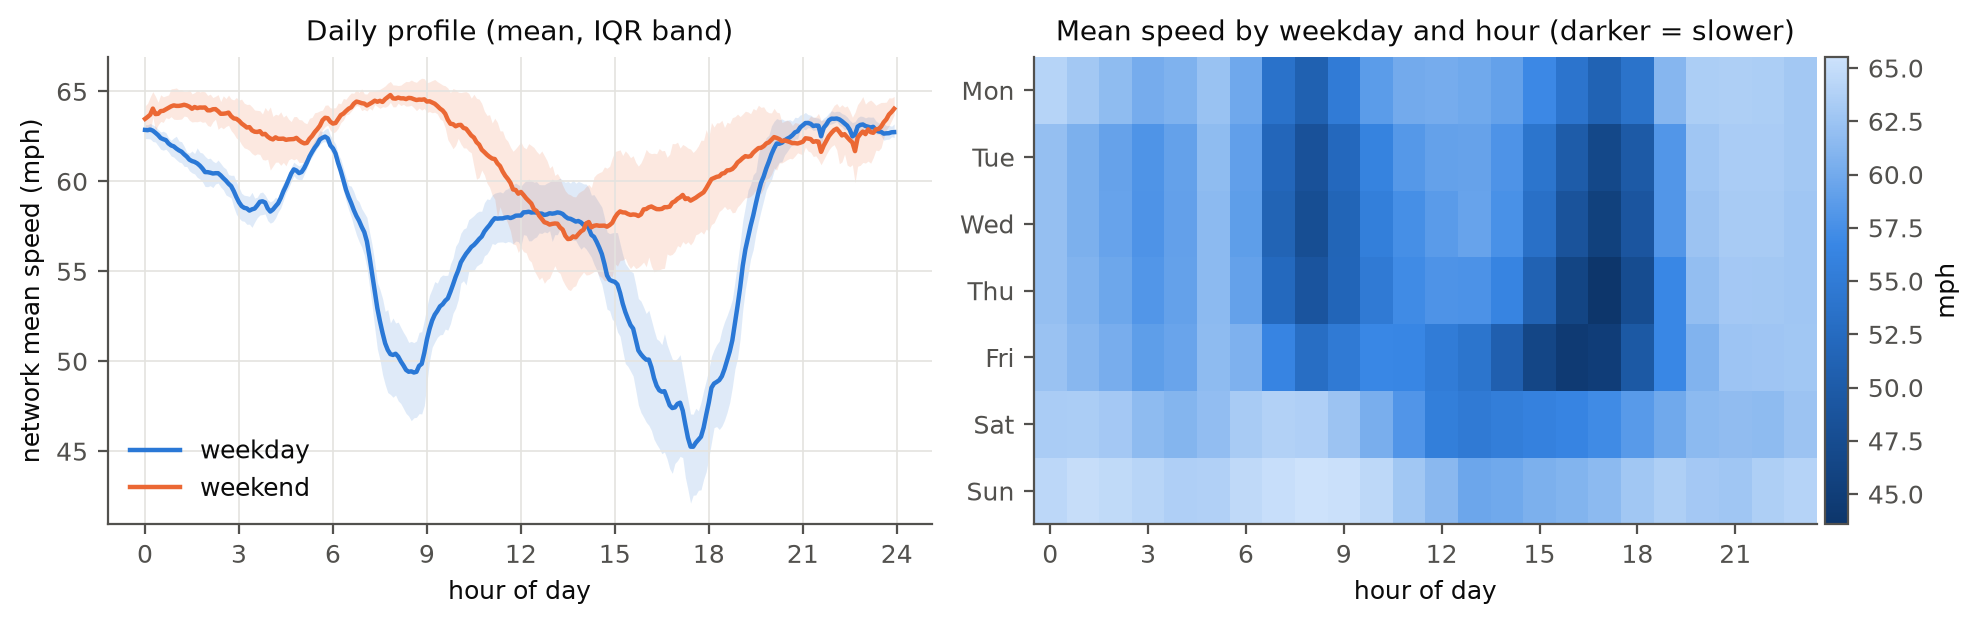
\includegraphics[width=0.9\textwidth]{eda_daily_profile.png}
\caption{Left: network-mean speed by time of day (line: mean; band: inter-quartile
range across days). Right: mean speed by weekday and hour.}
\label{fig:profile}
\end{figure*}

\begin{figure}[t]
\centering
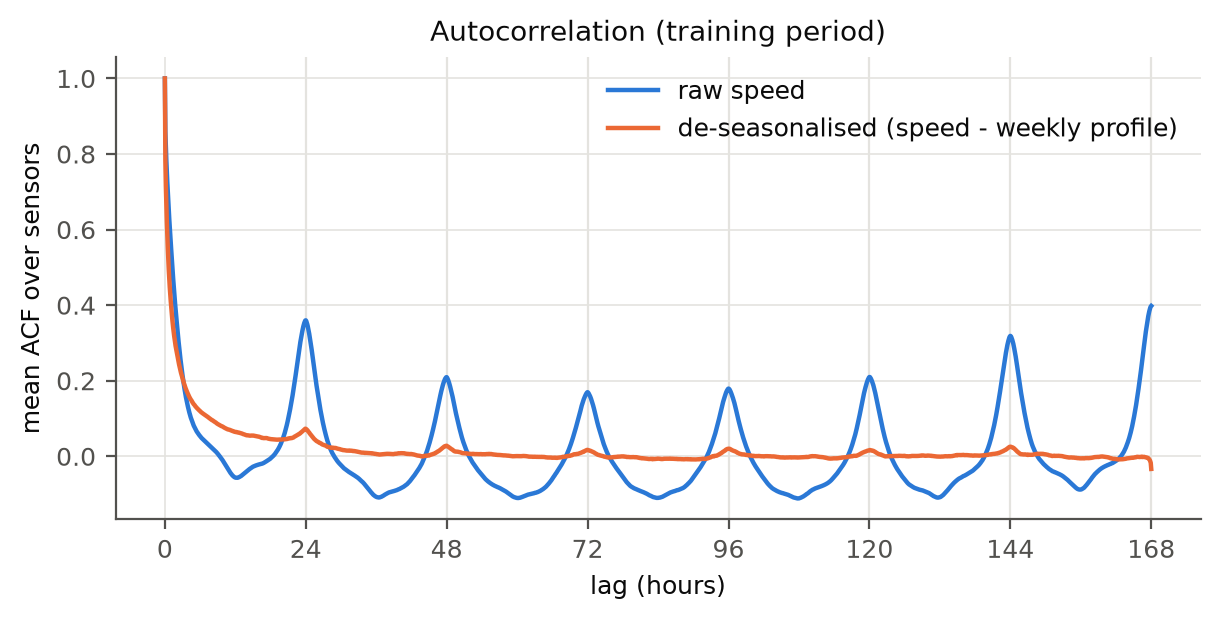
\includegraphics[width=\columnwidth]{eda_acf.png}
\caption{Mean autocorrelation over sensors, for raw speeds and after removing the
weekly profile.}
\label{fig:acf}
\end{figure}

\subsection{Spatial structure}
Pairwise correlation decays with road distance (Fig.~\ref{fig:spatial}), and the
decay persists after de-seasonalising, so it is not just a shared daily cycle.
Graph-connected sensors have a mean anomaly correlation of 0.27, against 0.07 for
pairs with no recorded road path. The Spearman correlation between distance and
anomaly correlation is $-0.20$. The distance graph is strongly directed: 73\,\%
of edges have no reverse edge, and five sensors have no outgoing edge. This
justifies both direction-aware spatial features and a learned adjacency.

\begin{figure}[t]
\centering
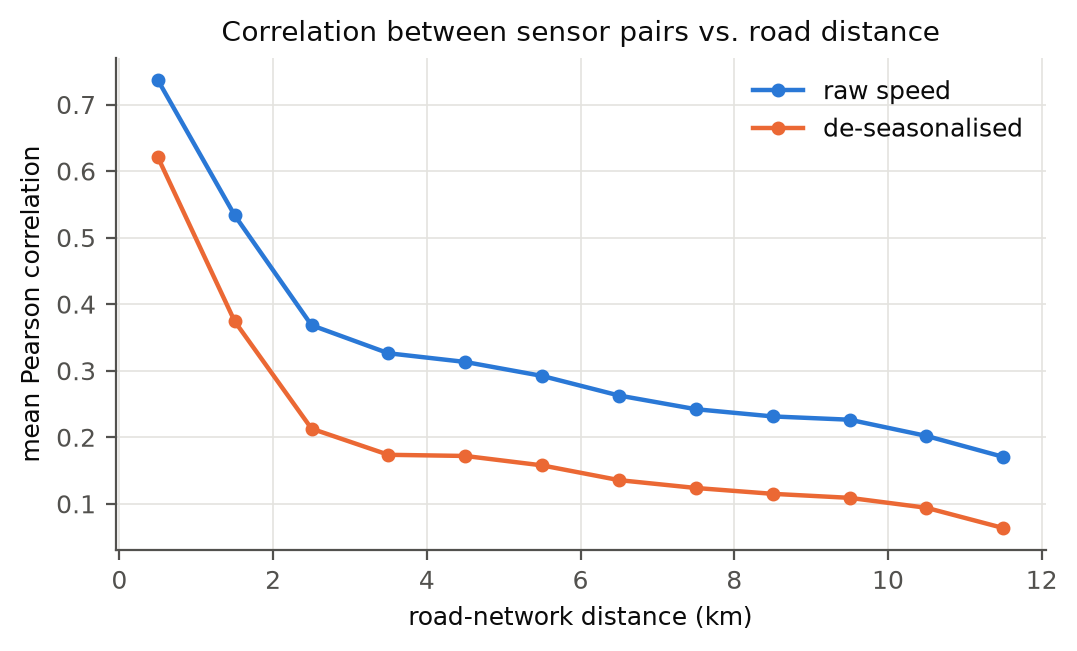
\includegraphics[width=\columnwidth]{eda_spatial_corr.png}
\caption{Mean Pearson correlation between sensor pairs, binned by road distance.}
\label{fig:spatial}
\end{figure}

\subsection{Split and distribution shift}
Following~\cite{li2018dcrnn,wu2019gwnet}, windows are split chronologically
70/10/20 (train to 23~May, validation to 4~June, test to 27~June). Mean speed is
stable across splits (58.6 / 58.9 / 57.8\,mph), but the test period has more missing
data (12.1\,\% vs.\ 7.1\,\% in training). This mild, realistic shift motivates the
robustness analysis in Section~\ref{sec:results}.
